\subsection{Архитектура на софтуерна програма}
Всяка софутерна програма изисква разработката на интерфейс, чрез който потребителя може да комуникира със програмата. Софтуерната програма е съставена от 4 модула, които комуникират помежду си, някои, от които имат визуална част, а други - не.
За разработката на софтуерната програма са използвани множество от практики за дизайн (design patterns), което позволява лесната поддръжка на софтуера за бъдеще \cite{patterns}.Имплементацията на модулите е реализирана чрез използването на широкоизползваната практика за дизайн - MVVM \cite{mvvm}. Предишната прекитка, предлага ясно разпределение между отговорностите на различните части на кода т.е код, които отговаря за логически операции не е свързан с код, който отговаря за обратната връзка между двете. Прадлага лесен начин за синхронизиране между логическата и визуалната част на дадена софтуерна програма чрез използване на "One way data binding" и "Two way data binding" похватите \cite{dataBinding}.

\begin{figure}
    \centerline{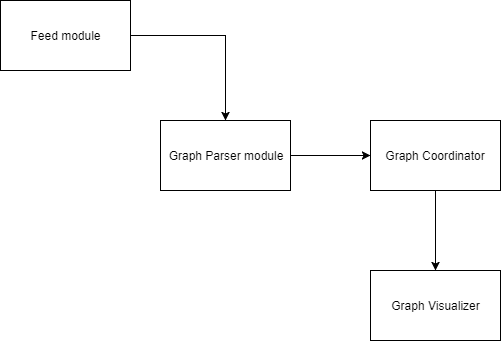
\includegraphics{modules}}
    \caption{Архитектура на софтуерната програма}
    \label{fig:architecture}
\end{figure}

\begin{itemize}
    \item Options модул, който предлага начин за модифициране на различни настройки свързани с начина на изобразяване на обектите и тяхната начална конфигурация.
    \item Connection модул, който позволява да се осъществява връзка между серийния порт и устройството
    \item Script модул, който позволява да се контролира скоростта на изпращане на информация от устройството към USB приемника.
    \item Feed  модул, който има за отговорност да захранва с данни останалите модули с граф, който за всяка точка съдържа разстояниято между точката и всички останали точки. Ако разстоянието между две точки не може да бъде измерено то тогава разстоянието се означава с специален флаг поле, което е дефинирано като -безкрайност.
    \item Graph Parser модул, който има за цел да обработи информацията, която ‘Feed’ модулът изпраща и да я трансформира в друг граф – който държи информацията във върхове и дъги. Върховете и дъгите съдържат информация, която помага за визуализацията на графа в 3D.
    \item Graph Coordinator модул, който има за цел да определи -координатите в пространството на всички обекти, които се съдържат в графа, който се получава в резултат на стъпка 2 (Graph Parser). Координатите се определят чрез система от линейни уравнения, които считат, че началната позиция на стационарните обекти е (0,0,0) - в един от ъглите на мястото, в което же бъдат следяни обектите.
    \item Graph Visualizer модул, който има за цел да използва графа, чиито координати са били вече определени от Graph Coordinator и да ги визуализира по удачен начин в 3 измерения.

\end{itemize}

\pagebreak

\subsection{Модул за опции}
Разработен е модул за опции, които позволява лесен контрол над началното разположение на статичните получатели в пространтвото. Модулът може да бъде използван чрез кликане на "Options" полето [фиг \ref{fig:options}]. Модулът изобразява презададен брой статични точки, чиито координати могат да бъдат зададени от потребителя на софтуерната програма. 

\begin{figure}
   \centerline{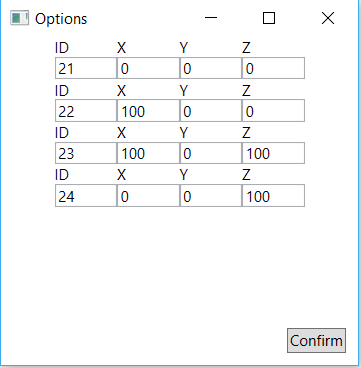
\includegraphics{options}}
    \caption{Меню за опции}
    \label{fig:options}
\end{figure}

\pagebreak

\subsection{Feed модул}
Feed модулът има за цел да създаде граф, който съдържа дистанциите от всяка точка до всяка друга. Нуждата от възможност за лесна и бърза смяна между двата подхода наложи създаването на модула.\\\\
В процеса на работа бяха изградени 2 различни начина за получаване на данните от ултразвук трансмитери към ултразвук получатели. 
\begin{enumerate}
    \itemДанните се получават директно от физическите обекти. Стандартното измерване се случва чрез получаване на данните през сериен порт. Данните се предоставят от ултразвукови трансмитери и получатели в специален формат, който бива преобразуван към граф, съдържащ разстоянията между различните точки. Данните се получават след като бъдат получени от Connection модула [сек. \ref{connModule}]
    \itemДанните биват генерирани чрез компютърен модел. Компютърния модел се състои от генератор на дистанции, който симулира движението на реален обект. Това се постига чрез манипулация на дистанцията между двойка (движещ,недвижещ) обект в пространството с константна стойност на определен интервал. Добавен е елемент на случайност, който позволява да се придаде по-реалистичен вид на движението на обектите.
\end{enumerate}

В програмният фрагмент по-долу е представена имплементацията на модула за захранване с данни. Изпраща се събитие за полученият граф на дистанциите.
\begin{lstlisting}
public void Push(Dictionary<string, List<Tuple<string, double>>> moving, Dictionary<string, List<Tuple<string, double>>> all)
{
    var movingData = new Dictionary<int, List<Tuple<int, double>>>();
    var staticData = new Dictionary<int, List<Tuple<int, double>>>();


    foreach (var node in moving)
    {
        movingData.Add(int.Parse(node.Key), node.Value.Select(x => new Tuple<int, double>(int.Parse(x.Item1), x.Item2)).ToList());
    }

    foreach (var node in all.Where(t => !moving.ContainsKey(t.Key)))
        staticData.Add(int.Parse(node.Key), node.Value.Select(z => new Tuple<int, double>(int.Parse(z.Item1), z.Item2)).ToList());

    DataReceived(this, new GraphArgs(staticData, movingData, nodes.ToList()));
}
\end{lstlisting}

\pagebreak

\subsection{Graph Parser модул}
Graph Parser модулът има за цел да използва графа генериран от Feed модулът, за да създаде граф на свързаност, който съдържа
\begin{enumerate}

\itemВърхове, които представляват движещи/недвижещи се обекти 

\itemДъги, свързващи върховете, които означават съществуването на свързаност между
даден връх и друг връх.\\

\end{enumerate}

В програмният фрагмент по-долу се създава двусвързан граф, който репрезентира обектите в пространството като върхове и разстоянията между тях като ребра.
\begin{lstlisting}
private IBidirectionalGraph<Vertex, Edge> ParseGraph(GraphArgs b)
{
    var graph = new BidirectionalGraph<Vertex, Edge>();

    var edgeQ = b.StaticVertices.Union(b.MovingTargets)
                                .ToDictionary(x => x.Key, y => y.Value);

    foreach (var node in b.StaticVertices)
    {
        var query = b.StaticNodes.FirstOrDefault(x => int.Parse(x.Id) == node.Key);
        graph.AddVertex(new Vertex(node.Key, true, new Vector3D(query.X, query.Y, query.Z)));
    }

    foreach (var node in b.MovingTargets)
        graph.AddVertex(new Vertex(node.Key, false));

    var vertices = graph.Vertices.ToList();

    foreach (var vertex in vertices)
    {
        foreach (var edge in edgeQ[vertex.ID])
        {
            var q = vertices.FirstOrDefault(x => x.ID == edge.Item1);
            if (q == null) continue;
            var e = new Edge(vertex, q)
            {
                Weight = edge.Item2
            };
            graph.AddEdge(e);
        }
    }

    return graph;
}
\end{lstlisting}

\pagebreak

\subsection{Graph Coordinator модул}
Целта на Graph Coordinator модула е да определи координатите в 3D на построения граф. Тази операция се извършва чрез минимизиране на бройката на възможните позиции използвайки система от уравнения. Всички възможни позиции се намират на радиус с дължина R (равен на дистанцията получена от сензора) на сфера. Задачата се трансформира:\\

\textit{За всеки получател се образуват K сфери (K=броя на трансмитерите), като сфера $x_i$ се центрира в позицията на на трансмитер с индекс $i$, а радиусът и е равен на измерената стойност за разстоянието между двата обекта. За да получим еднозначно решение ние трябва да елиминираме всички възможни позиции освен една. Всички решения на задачата за даден получател се намират на пресечния регион на всички сфери за дадения получател. Търси се такава конфигурация на позициите на всички получатели така че назначените позиции да не са в конфликт и броят на възможни решения за всяка позиция да е минимален.}\\\\

В 2D намирането на решения е лесно, поради следните причини:

\begin{enumerate}
    \itemБроят на пресечните точки на сферите при оптимално* позициониране на сензорите лесно може да бъде сведено до еднозначно решение.

    \itemВ 2-D пресечните точки на окръжностите са точки. В 3D пресечните точки се описват от 3D фигура. Това лесно може да бъде видяно на фигура \ref{spheres}.
\end{enumerate}
\begin{figure}
    \centerline{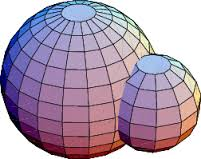
\includegraphics{spheres}}
    \caption{Пресечната точка на сфери в 3D е 3D регион от точки}
    \label{spheres}
\end{figure}


В софтуерната програма разработена като приложение към текущата дипломна работа е имплементиран метод за определяне на позицията на обекти, които могат да се движат в пространството. В програмният фрагмент по-долу, имплементиран на програмния език C#, е представен математическият апарат за намирането на координатите в тримерна декартова система на подвижната точка, като се използва система от линейни уравнения. 

\begin{lstlisting}
/// <summary>
/// Determine coordinates of 'vertex' relative to the state of 'graph'
/// </summary>
/// <param name="vertex"></param>
/// <param name="graph"></param>
private void DeterminePosition(Vertex vertex, IBidirectionalGraph<Vertex, Edge> graph)
{
    if (vertex.IsReceiver) return;
    if (graph.VertexCount != 5) return;

    // Get the points
    var points = graph.Vertices.Where(n => n.IsReceiver).OrderBy(n => n.ID).ToList();

    var d21 = Euclidean(points[1].Position, points[0].Position);
    var d31 = Euclidean(points[2].Position, points[0].Position);
    var d41 = Euclidean(points[3].Position, points[0].Position);

    // Get the edges
    Edge e;
    if (!graph.TryGetEdge(vertex, points[0], out e)) return;
    var r1 = e.Weight;
    if (!graph.TryGetEdge(vertex, points[1], out e)) return;
    var r2 = e.Weight;
    if (!graph.TryGetEdge(vertex, points[2], out e)) return;
    var r3 = e.Weight;
    if (!graph.TryGetEdge(vertex, points[3], out e)) return;
    var r4 = e.Weight;

    var b21 = (Math.Pow(r1, 2) - Math.Pow(r2, 2) + Math.Pow(d21, 2)) / 2;
    var b31 = (Math.Pow(r1, 2) - Math.Pow(r3, 2) + Math.Pow(d31, 2)) / 2;
    var b41 = (Math.Pow(r1, 2) - Math.Pow(r4, 2) + Math.Pow(d41, 2)) / 2;

    // System of equations
    var A = Matrix<double>.Build.DenseOfArray(new double[,]
    {
        {points[1].Position.X-points[0].Position.X,points[1].Position.Y - points[0].Position.Y,points[1].Position.Z-points[0].Position.Z },
        {points[2].Position.X-points[0].Position.X,points[2].Position.Y - points[0].Position.Y,points[2].Position.Z-points[0].Position.Z },
        {points[3].Position.X-points[0].Position.X,points[3].Position.Y - points[0].Position.Y,points[3].Position.Z-points[0].Position.Z }
    });
    
    
    var B = Vector<double>.Build.Dense(new double[] { b21, b31, b41 });
    
    // Solve the system
    var X = A.Solve(B);

    // Normaization
    var finalPosition = NormalizePosition(points, X);
    
    //set the final position
    vertex.Position = new Point3D(finalPosition.X, finalPosition.Y, finalPosition.Z);
}
\end{lstlisting}

Разработен е метод за нормализация на разстоянието, който води до по-коректно изобразяване на данните тъй като в резултат на работата с приблизителни разстояния предоставени от сензорите.В програмният фрагмент по-долу е представен авторова интерпретация на метод за нормализация на координатите на движеща се точка. Чрез периодични измервания с използвания хардуер е определен параметър, който води до най-добри резултати във визуализацията. За да се нормализира успешно позицията се намира центъра на равнината \cite{centroid}, в която са позиционирани всички статични сензори ( счита се, че сензорите са в една равнина) с помощта на следната формула :

\centerline{\begin{equation}
    
\end{equation}}

\begin{lstlisting} \label{normalize}
/// <summary>
/// A method for normalization based on empirical studies of the output for the current sensor
/// </summary>
/// <param name="points">Static points</param>
/// <param name="X">The determined position of the point</param>
/// <returns></returns>
private static Vector3D NormalizePosition(List<Vertex> points, Vector<double> X)
{
    var vectPoint = new Vector3D(X[0], X[1], X[2]);
    
    //Transform the static points to vectors
    var vectors = new[] { points[0], points[1], points[2], points[3] }
                        .Select(n => new Vector3D(n.Position.X, n.Position.Y, n.Position.Z)).ToList();

    // Find the middle point of the static points
    var mid = vectors.Aggregate((curr, next) => { return curr += next; }) / vectors.Count;
    // Find a vector from the mid to the target position
    var midToPoint = mid - vectPoint;
    var length = midToPoint.Length;

    //normilized vector
    midToPoint.Normalize();

    //Increase the vector by the determined factor
    var final = midToPoint * (0.0001 * length);
    return final;
}
\end{lstlisting}

\pagebreak



\subsection{Connection модул}\label{connModule}
Свързването с хардуерно устройство, от което могат да се получават данни е задача, която е решена чрез разработка на connection модул за софутерната програма [фиг. \ref{fig:connection}]. Както може да се види на фигурата потребителя избира серийния порт поле Serial Port в случая COM3 и скоростта на обмен на данни поле Bauld Rate в случая 256000.

Програмният фрагмент по-долу се изпълнява в конструктора и служи за взимане на текущо наличните серийни портове на компютъра, след което се избира първият намерен.
\begin{lstlisting}
// Constructor
public SerialInterface()
{
    // Finding installed serial ports on hardware
    _currentSerialSettings.PortNameCollection = SerialPort.GetPortNames();
    _currentSerialSettings.PropertyChanged += new \\System.ComponentModel.PropertyChangedEventHandler(_currentSerialSettings_PropertyChanged);

    // If serial ports is found, we select the first found
    if (_currentSerialSettings.PortNameCollection.Length > 0)
        _currentSerialSettings.PortName = _currentSerialSettings.PortNameCollection[0];
}
\end{lstlisting}



\begin{figure}
    \centerline{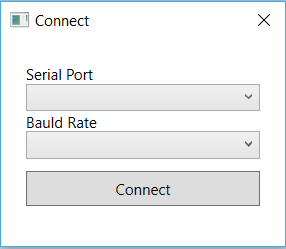
\includegraphics{connect}}
    \caption{Connection модул}
    \label{fig:connection}
\end{figure}

\subsection{Script execution module}
За да може да бъде конфигурирано по-време на използване на софтуерната програма използваното устройство [фиг.\ref{fig:device}] има нужда да може да получава команди, които да бъдат подадени от програмата. За да се реши този проблем е разработен модул, който позволява изпращането на инструкции, които контролират скоростта на предаване на данни от устройствотo [фиг.\ref{fig:script}].
\\
В програмният фрагмент по-долу е представена реализацията на изпращането на скрипта към серийния порт:
\begin{lstlisting}
// Execute Button
        private void Execute_Button_Click(object sender, RoutedEventArgs e)
        {
            try
            {
                string[] lines = Regex.Split(Scrypt.Text, "\r\n");
                foreach (var line in lines)
                {                    
                    if (line.Length == 0) continue; // empty line                    
                    if (line.Substring(0, 1) == "#") continue; // comment line
                    string command = CheckSum(line,'\n');
                    _port.Send(command); 
                    Thread.Sleep(200); 
                }
                MessageBox.Show("Script Send Successful!", "Information", MessageBoxButton.OK, MessageBoxImage.Information);
            }
            catch (Exception Error)
            {
                MessageBox.Show(Error.Message, "Error", MessageBoxButton.OK, MessageBoxImage.Error);
            }
        }
\end{lstlisting}




\begin{figure}
    \centerline{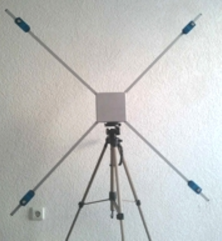
\includegraphics{device}}
    \caption{Hexamite устройството изпозлвано в тестването}
    \label{fig:device}
\end{figure}

\begin{figure}
    \centerline{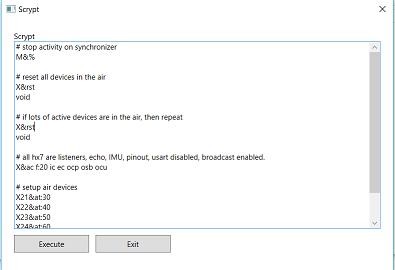
\includegraphics{script}}
    \caption{Модул за изпращане на инструкции}
    \label{fig:script}
\end{figure}

\subsection{Graph Visualizer модул}
Целта на Graph Visualizer модула е да използва графа, чиито координати са били вече определени от Graph Coordinator и да ги визуализира по удачен начин в 3 измерения.\\
В програмният фрагмент по-долу служи за визуализация на върхове и ребра, като за неговата работа се изисква използване на входен параметър представляващ пълния ориентиран свързан граф.

На [Фиг. \ref{fig:visualize}] е представена визуализация на примерен граф с 4 стационарни точки и 1 подвижна точки, като данните се получават в реално време от ултразвуковата апаратна част.
\begin{figure}
    \centerline{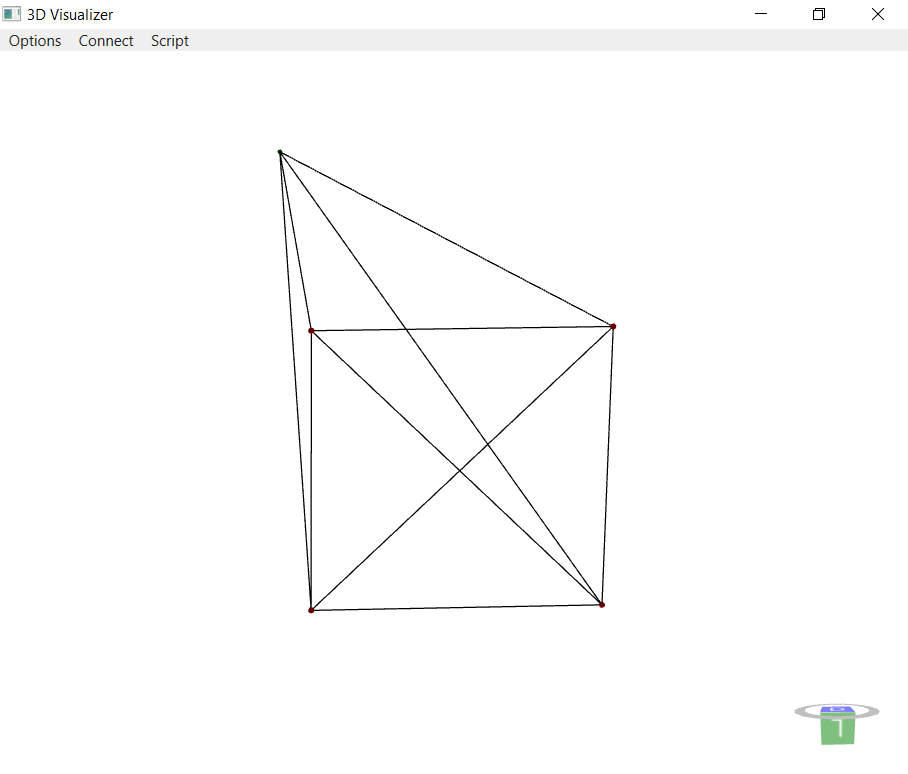
\includegraphics{visualize}}
    \caption{Визуализация на графа}
    \label{fig:visualize}
\end{figure}


\begin{lstlisting}
/// <summary>
/// Load visual models
/// </summary>
/// <param name="graph"></param>
public void Load(IBidirectionalGraph<Vertex, Edge> graph)
{
    Models.Clear();
    _vertexVisuals.Clear();
    _edgeVisuals.Clear();

    Models.Add(new SunLight());

    foreach (var node in graph.Vertices)
    {
        SphereVisual3D visual;
        Models.Add(visual = new SphereVisual3D()
        {
            Center = node.Position,
            Radius = 10,
            Fill = node.IsReceiver ? Brushes.Red : Brushes.Green,
            BackMaterial = new DiffuseMaterial(Brushes.Red)
        });
        _vertexVisuals.Add(node, visual);
    }

    foreach (var edge in graph.Edges)
    {
        if (!double.IsNegativeInfinity(edge.Weight))
        {
            LinesVisual3D lv3;
            Models.Add(lv3 = new LinesVisual3D()
            {
                Points = new Point3DCollection()
                {
                    edge.Source.Position,
                    edge.Target.Position
                }
            });
            _edgeVisuals.Add(edge, lv3);
        }
    }
}
\end{lstlisting}



\subsection{Обобщение}
Разработена е архитектура за софтуерно решение за платформа за визуализация на ултразвукови компоненти в 3 измерения. 